\begin{frame}
  \begin{columns}
    \column{0.5\textwidth}
    \frametitle{Sistemas de diálogo Humano-Computadora}
    \framesubtitle{Ejemplos de ``falta de naturalidad''}

    Relativamente bien en lo lingüístico, pero mal en las emociones, actitudes, intenciones, etc.

    Ejemplos:
    \begin{enumerate}
      \item Sistemas telefónicos
      \item Apple Siri
      \item Google Now
      \item Amazon Echo
      \item Microsoft Cortana
      \item HAL 9000
    \end{enumerate}
    \column{0.5\textwidth}
    \begin{figure}
      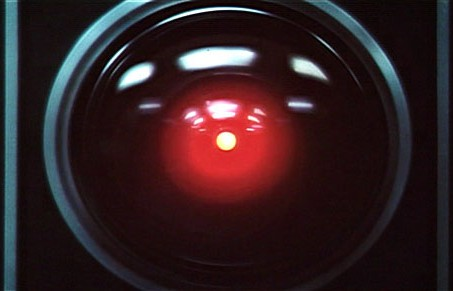
\includegraphics[scale=0.35]{images/hal.jpg}
    \end{figure}
  \end{columns}
\end{frame}

\begin{frame}
  \frametitle{Mimetización}
  \begin{itemize}
    \item Mimetización: Fenómeno insconsciente que se manifiesta a través de la adaptación de los hablantes. Fuertemente emparentada con el sentimiento de empatía.
    \item Objetivo del trabajo: Explorar, refinar y validar una métrica de la mimetización acústico-prosódica.
  \end{itemize}

\end{frame}

\section{Introducción}

\subsection{Prosodia}

\begin{frame}
  \frametitle{Prosodia}
  \framesubtitle{¿Qué es?}
  \begin{itemize}
    \item El ``cómo'' decimos las cosas, a diferencia del ``qué''
    \item Parte fundamental de la comunicación oral.
    \item Características que la definen: acentuación, velocidad, tono, ritmo, volumen.
    \item Una de las principales fallas en los sistemas humano-computadoras hoy día
    \item Transmite emociones, actitudes, y también desambigua.
    \item Ej. de desambiguación: ``Hola, qué pasa?''
  \end{itemize}

  \vfill
\end{frame}


\subsection{Mimetización}

\begin{frame}
  \frametitle{Mimetización}
  \framesubtitle{¿Qué es?}
  \begin{columns}
  \column{0.40\textwidth}
    \begin{figure}
      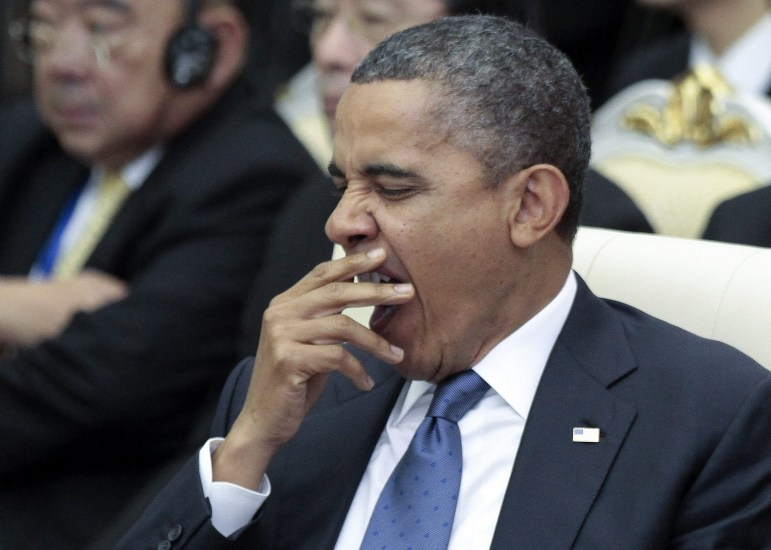
\includegraphics[width=\textwidth]{images/bostezo.jpg}
    \end{figure}

  \column{0.60\textwidth}
  \begin{enumerate}
    \item También conocida como entrainment, convergencia, efecto camaleón, etc.
    \item Adaptación que ocurre entre hablantes a varios niveles: sintáctico, prosódico, en las posturas, etc.
    \item Fenómeno ubicuo e inconsciente en la comunicación humana
    \item Para el presente trabajo, sólo nos interesa medir la \textbf{mimetización acústico-prosódica} sobre variables como el tono o pitch, volumen, calidad de habla, y otras.

  \end{enumerate}

  \end{columns}

\end{frame}

\begin{frame}
  \frametitle{Mimetización}
  \framesubtitle{¿Y cómo la medimos?}

  \begin{itemize}
    \item La definición de mimetización hasta acá vista es muy subjetiva ¿Cómo definimos una medida para esto?
    \item Vamos a explorar una métrica definida en trabajos anteriores, pulirla un poco, y verificar que efectivamente capture ciertas características del mimetización.
    \item ¿Cómo? Aplicándola a un corpus con anotaciones sociales, y verificando la relación entre las percepciones sociales y la métrica del \emph{mimetización}
  \end{itemize}


\end{frame}
